\documentclass{beamer}
\usetheme{metropolis}
\usepackage{graphicx}
\usepackage{subcaption}
\usepackage{hyperref}
\usepackage{tcolorbox}
\title{Algebra-Based Physics-1: Mechanics (PHYS135A-01): Week 7}
\date{October 16th - October 20th, 2017}
\author{Jordan Hanson}
\institute{Whittier College Department of Physics and Astronomy}

\begin{document}
\maketitle

\section{Week 6 Review}

\begin{frame}{Week 6 Review}
\begin{enumerate}
\item \alert{Angular} kinematics and dynamics
\begin{itemize}
\item Angular displacement
\item Angular velocity
\item Centripetal acceleration
\end{itemize}
\item \alert{Newton's Law of Gravity} and circular orbits
\item Kepler's Laws
\end{enumerate}
\end{frame}

\section{Week 6 Review Problem}

\begin{frame}{Week 6 Review Problem}
On the game show Wheel of Fortune, a large wheel is divided into sections worth varying dollar amounts.  Contestants try to spin the wheel such that they get the good ones.  Player 1 notices that the \$10,000 marker is on the opposite side (180 degrees away).  What is this angle in radians?  If she has great luck and spins such that the wheel turns exactly 180 degrees, in 2 seconds, what is the angular speed in radians per second?
\begin{itemize}
\item A: $\pi/2$ radians, $\pi/4$ radians per second
\item B: $0$ radians, $0$ radians per second
\item C: $\pi$, $\pi/2$ radians per second
\item D: $\pi$, $\pi/4$ radians per second
\end{itemize}
\end{frame}

\begin{frame}{Week 6 Review Problem}
Astronomers are observing two planets orbiting a star for several months.  They observe that planet 1 orbits twice as fast as planet 2.  If the orbital radius of planet 1 is 1 AU, what is the orbital radius of planet 2, in AU?
\begin{itemize}
\item A: 1 AU
\item B: 1.6 AU
\item C: 4 AU
\item D: 3.2 AU
\end{itemize}
\end{frame}

\section{Week 7 Summary}

\begin{frame}{Week 7 Summary}
\begin{enumerate}
\item \alert{Work} has a scientifically precise definition
\item Kinetic Energy and the \alert{Work-Energy Theorem}
\begin{enumerate}
\item Reduces complexity in problem solving
\item Interested in only initial and final \textit{states}
\end{enumerate}
\item Gravitational potential energy
\item Definition of a \textbf{conservative force} and potential energy
\end{enumerate}
\end{frame}

\section{Definition of Work}

\begin{frame}{Definition of Work}
\begin{tcolorbox}[colback=white,colframe=red!40!blue,title=Definition of Work]
\small
\alert{
The work done on a system by a constant force is the product of the component of the force in the direction of motion times the distance through which the force acts.  For one-way motion in one dimension, this is expressed in equation form as 
\begin{equation}
W = Fd\cos\theta = \vec{F} \cdot \vec{d}
\end{equation}
where $W$ is work, $F$ is the magnitude of the force on the system, $d$ is the magnitude of the displacement of the system, and $\theta$ is the angle between the force vector $F$ and the displacement vector $d$.
}
\end{tcolorbox}
\end{frame}

\begin{frame}{Definition of Work}
\begin{figure}
\centering
\begin{subfigure}{0.3\textwidth}
\centering
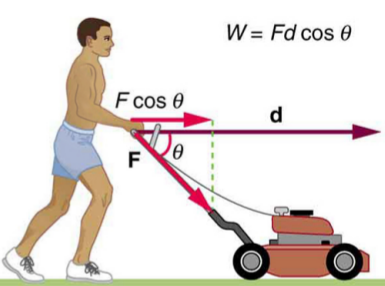
\includegraphics[width=\textwidth]{figures/lawn1.png}
\caption{}
\end{subfigure}
\begin{subfigure}{0.135\textwidth}
\centering
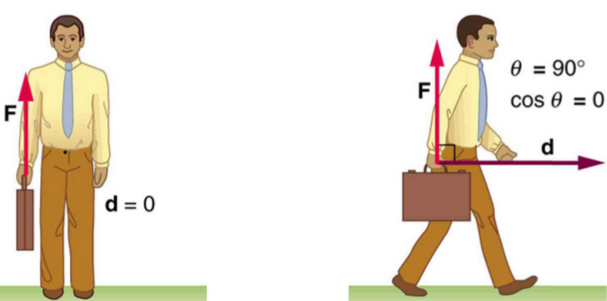
\includegraphics[width=\textwidth,trim=0cm 0cm 15cm 0cm,clip=true]{figures/lawn2.png}
\caption{}
\end{subfigure}
\begin{subfigure}{0.2\textwidth}
\centering
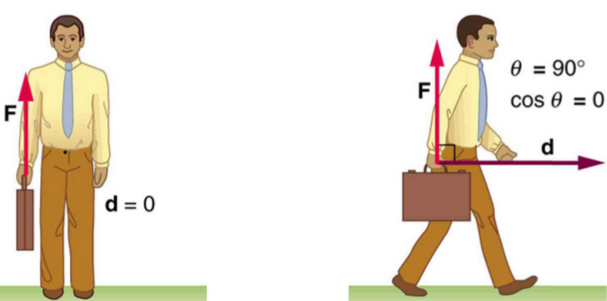
\includegraphics[width=\textwidth,trim=12cm 0cm 0cm 0cm,clip=true]{figures/lawn2.png}
\caption{}
\end{subfigure}
\begin{subfigure}{0.45\textwidth}
\centering
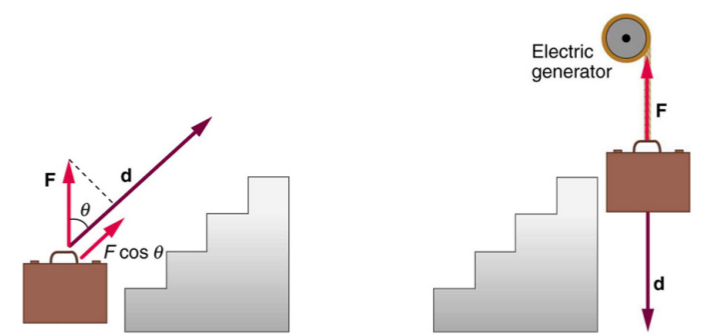
\includegraphics[width=\textwidth]{figures/lawn3.png}
\caption{}
\end{subfigure}
\caption{\label{fig:workvisual}\small (a) General case of work (b) No work, $d=0$ (c) No work, $\vec{F}\cdot\vec{d}=0$ (d) Positive work, then negative work}
\end{figure}
\end{frame}

\begin{frame}{Definition of Work}
Work has the unit of the \textit{Joule}, which is denoted \\ \textbf{1 J = 1 N m, or 1 kg m$^2$ s$^{-1}$.} \\  \vspace{1cm}
\small
\alert{Just in case people didn't hear this the first time...}\\
\textit{Extra credit opportunity}: \textbf{Do you like beer}?  Write a 10-page paper on the on the scientific challenge faced by James Prescott Joule, who began to formulate the modern view of energy in the 19th century, contrary to \textit{caloric theory}.  \textbf{Upon completion of this assignment I will change the lowest midterm score to a perfect score.}
\end{frame}

\begin{frame}{Definition of Work}
\begin{figure}
\centering
\begin{subfigure}{0.12\textwidth}
\centering
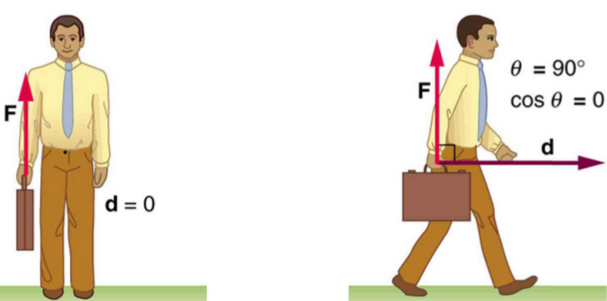
\includegraphics[width=\textwidth,trim=0cm 0cm 15cm 0cm,clip=true]{figures/lawn2.png}
\caption{}
\end{subfigure}
\begin{subfigure}{0.18\textwidth}
\centering
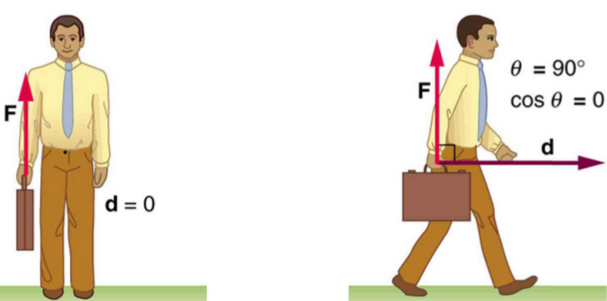
\includegraphics[width=\textwidth,trim=12cm 0cm 0cm 0cm,clip=true]{figures/lawn2.png}
\caption{}
\end{subfigure}
\begin{subfigure}{0.43\textwidth}
\centering
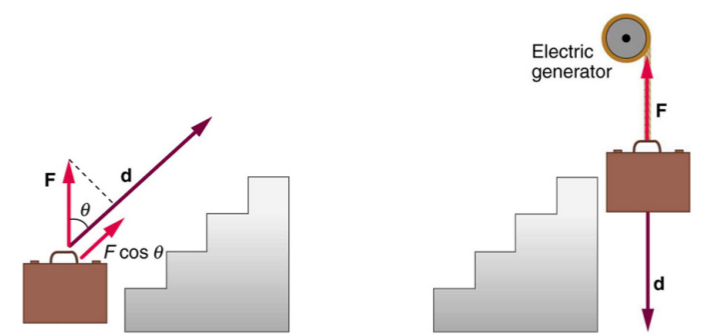
\includegraphics[width=\textwidth]{figures/lawn3.png}
\caption{}
\end{subfigure}
\caption{\label{fig:workvisual2} Different cases involving work.}
\end{figure}
\small
Rank the work done \textit{on the briefcase by F} from greatest to least.
\begin{itemize}
\item A: Case C (left) > Case A = Case B > Case C (right)
\item B: Case C (right) > Case A = Case B > Case C (left)
\item C: Case C (left) > Case A > Case B > Case C (right)
\item D: Case C (left) > Case B > Case A > Case C (right)
\end{itemize}
\end{frame}

\begin{frame}{Definition of Work}
\begin{figure}
\centering
\begin{subfigure}{0.3\textwidth}
\centering
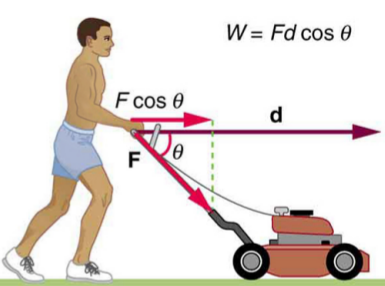
\includegraphics[width=\textwidth]{figures/lawn1.png}
\caption{}
\end{subfigure}
\begin{subfigure}{0.135\textwidth}
\centering
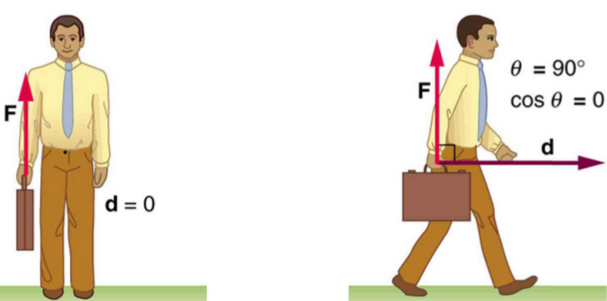
\includegraphics[width=\textwidth,trim=0cm 0cm 15cm 0cm,clip=true]{figures/lawn2.png}
\caption{}
\end{subfigure}
\begin{subfigure}{0.2\textwidth}
\centering
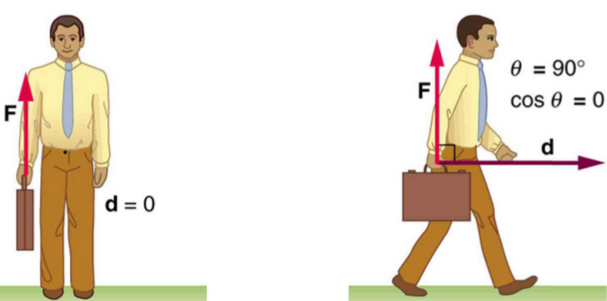
\includegraphics[width=\textwidth,trim=12cm 0cm 0cm 0cm,clip=true]{figures/lawn2.png}
\caption{}
\end{subfigure}
\caption{\label{fig:workvisual3} Different cases involving work.}
\end{figure}
\small
Rank the work \textit{on the mower/briefcase by F} from greatest to least.
\begin{itemize}
\item A: Case C > Case B > Case A
\item B: Case B = Case C > Case A
\item C: Case A > Case B = Case C
\item D: Case A = Case B = Case C
\end{itemize}
\end{frame}

\begin{frame}{Definition of Work}
\begin{figure}
\centering
\begin{subfigure}{0.3\textwidth}
\centering
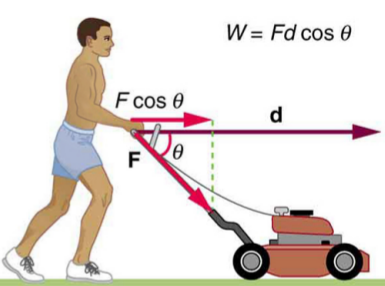
\includegraphics[width=\textwidth]{figures/lawn1.png}
\caption{}
\end{subfigure}
\begin{subfigure}{0.2\textwidth}
\centering
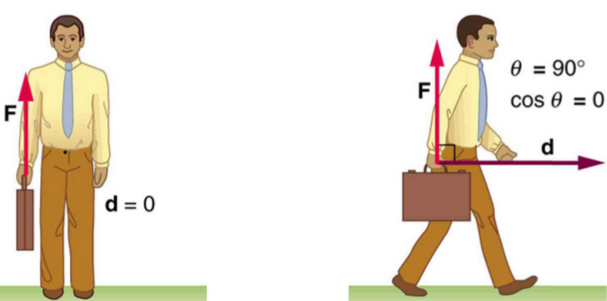
\includegraphics[width=\textwidth,trim=12cm 0cm 0cm 0cm,clip=true]{figures/lawn2.png}
\caption{}
\end{subfigure}
\caption{\label{fig:workvisual4} Different cases involving work.}
\end{figure}
\small
Which changes would \textit{increase} the work in both Case A and Case B?
\begin{itemize}
\item A: Case A: decrease $\theta$, Case B: decrease $\theta$.
\item B: Case A: increase $\theta$, Case B: decrease $\theta$.
\item C: Case A: decrease $\theta$, Case B: increase $\theta$.
\item D: Case A: increase $\theta$, Case B: increase $\theta$.
\end{itemize}
\end{frame}

\begin{frame}{Definition of Work}
Suppose a system is displaced by $\vec{d} = 2\hat{i}-3\hat{j}$ m by a force $\vec{F} = -3\hat{i}+5\hat{j}$ N.  What is the work done on the system by $\vec{F}$?
\begin{itemize}
\item A: 21 N
\item B: -21 N
\item C: 15 N
\item D: -15 N
\end{itemize}
\end{frame}

\begin{frame}{Definition of Work}
Suppose a system is displaced by $\vec{d} = 2\hat{i}-3\hat{j}$ m \textit{against} a force $\vec{F} = -3\hat{i}+5\hat{j}$ N.  What is the work done on the system by $\vec{F}$, if the system moves at constant velocity?
\begin{itemize}
\item A: 21 N
\item B: -21 N
\item C: 15 N
\item D: -15 N
\end{itemize}
\end{frame}

\begin{frame}{Definition of Work}
As we will see, work is a form of \textit{energy}.  There are other units of energy which apply to different \textit{energy scales}.  A human being requires about 2000 kcal of food energy per day.  If 1 kcal equals 1000 calories, and 1 calorie equals 4.184 J, how many Joules of energy does one human require per day?
\begin{itemize}
\item A: 1 kJ (a thousand Joules)
\item B: 10 kJ (ten thousand Joules)
\item C: 1 MJ (a million Joules)
\item D: 10 MJ (ten million Joules) 
\end{itemize}
\end{frame}

\begin{frame}{Definition of Work}
Calculate the mass of an object displaced 1 meter ($d = 1\hat{j}$) \textit{against} gravity, $F = -mg\hat{j}$, if the work done was equal to 10 MJ.
\begin{itemize}
\item A: 1000 kg
\item B: 10,000 kg
\item C: 100,000 kg
\item D: 1,000,000 kg
\end{itemize}
\textit{Our bodies burn a lot of energy...we will return to this!}
\end{frame}

\begin{frame}{Definition of Work}
\begin{figure}
\centering
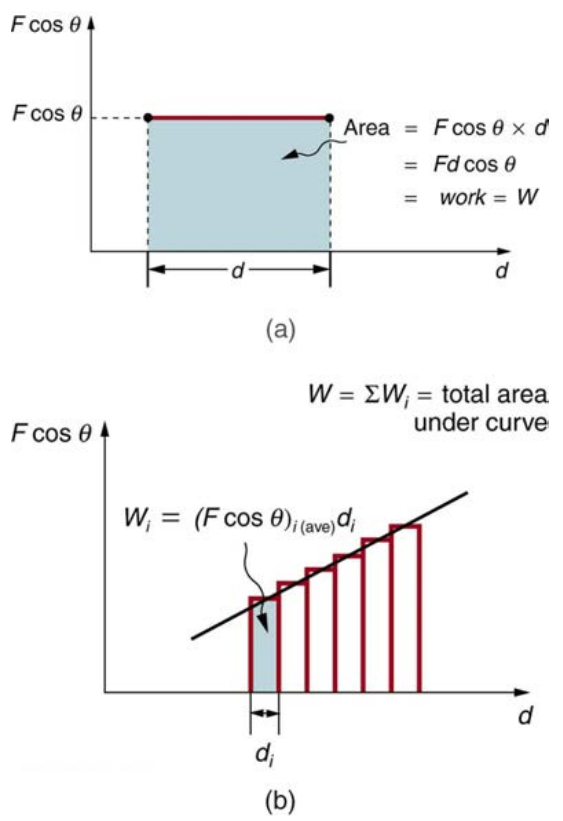
\includegraphics[width=0.4\textwidth]{figures/area.png}
\caption{\label{fig:area} Generally, work is the area under a curve of force applied versus displacement.}
\end{figure}
\end{frame}

\begin{frame}{Definition of Work}
Suppose a 100 kg system is displaced 5 m through a region with kinetic friction coefficient of 0.02, and then displaced by 10 m through a region with kinetic friction coefficient 0.01.  What is the work done on the system?
\begin{itemize}
\item A: 10 J
\item B: 20 J
\item C: 100 J
\item D: 200 J
\end{itemize}
\end{frame}

\begin{frame}{Definition of Work}
Notice from this problem, that we had to discover an equation: $W = \mu m g d$.  This is the work done against friction when friction is the net force, and $d$ is the displacement. \\ \vspace{1cm}
\textbf{Work against friction net force:}
\begin{equation}
W = \mu m g d
\end{equation}
\end{frame}

\section{Kinetic Energy and the Work-Energy Theorem}

\begin{frame}{Kinetic Energy and the Work-Energy Theorem}
\begin{tcolorbox}[colback=white,colframe=red!40!blue,title=The Work-Energy Theorem]
\small
\alert{
Let the \textit{kinetic energy} of a system with mass $m$ be defined to be $KE = \frac{1}{2}mv^2$.  The work done on a system is equal to the change in kinetic energy:
\begin{equation}
W = KE_{\rm f} - KE_{\rm i} = \Delta KE
\end{equation}
}
\end{tcolorbox}
\end{frame}

\begin{frame}{Kinetic Energy and the Work-Energy Theorem}
\end{frame}

\section{Conclusion}

\begin{frame}{Week 7 Summary}
\begin{enumerate}
\item \alert{Work} has a scientifically precise definition
\item Kinetic Energy and the \alert{Work-Energy Theorem}
\item Gravitational potential energy
\item Definition of a \textbf{conservative force} and potential energy
\end{enumerate}
\end{frame}

\section{Answers}

\begin{frame}{Answers}
\begin{columns}[T]
\begin{column}{0.5\textwidth}
\begin{itemize}
\item $\pi$, $\pi/2$ radians per second
\item 1.6 AU
\item Case C (left) > Case A = Case B > Case C (right)
\item Case A > Case B = Case C
\item Case A: decrease $\theta$, Case B: decrease $\theta$.
\item -21 N
\item 21 N
\item 10 MJ (ten million Joules)
\item 1,000,000 kg
\item 200 J
\end{itemize}
\end{column}
\begin{column}{0.5\textwidth}
\begin{itemize}
\item ... 
\end{itemize}
\end{column}
\end{columns}
\end{frame}

\end{document}
